% Generated by tex/build_swebok_structure.py from tex/chapters/ch01/07_要求妥当性確認.tex
\subsubsection{プロトタイピング}

\term{プロトタイプ}とは、本格的な実装の前に作る試作品である。画面の動き、操作感、処理の流れ、重要な技術的可能性などを具体的に示すために使う。

プロトタイプは、技術者の解釈を利害関係者に見せ、誤解を早く発見するのに有効である。ただし、見た目の細部や一時的な品質問題に関心が向きすぎると、本来確認したい要求から注意がそれることがある。

\begin{figure}[htbp]
\centering
\IfFileExists{swebok_structure/CH01.ソフトウェア要求(Software_Requirements)/1.5.要求妥当性確認(Requirements_Validation)/1.5.3.プロトタイピング(Prototyping)/assets/fig-ch01-09.png}{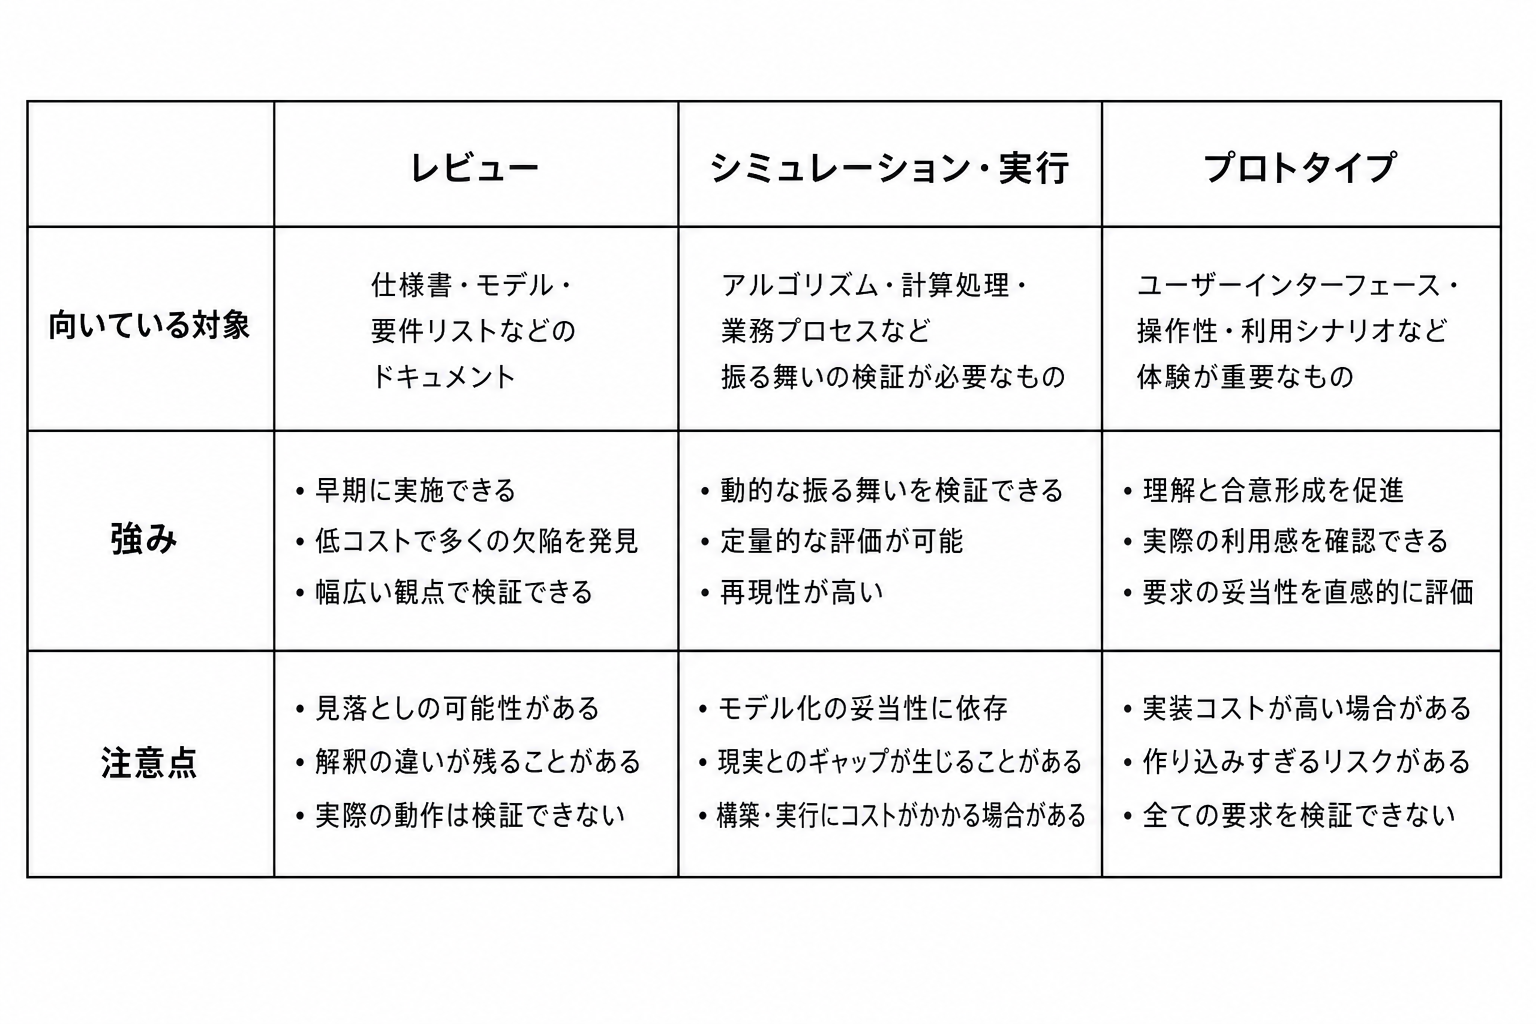
\includegraphics[width=0.96\linewidth]{swebok_structure/CH01.ソフトウェア要求(Software_Requirements)/1.5.要求妥当性確認(Requirements_Validation)/1.5.3.プロトタイピング(Prototyping)/assets/fig-ch01-09.png}}{\fbox{\parbox[c][48mm][c]{0.9\linewidth}{\centering 画像生成待ち\\要求妥当性確認の三手法を比較する図}}}
\caption{要求妥当性確認の三手法を比較する図}
\label{fig:ch01-09}
\end{figure}
